\documentclass{beamer}

\usepackage[utf8]{inputenc}
\usecolortheme{beaver}
\usepackage{caption}
\usepackage{subcaption}
\usepackage{mathtools}
\usepackage{todonotes}
\usepackage{amsmath}
\usepackage{bm}
\usepackage{listings}
\usepackage{ragged2e}
\usepackage{titlecaps}
\usepackage{fancyvrb}

\def\ci{\perp\!\!\!\!\!\perp}

\newtheorem{proposition}{Proposition}
\Addlcwords{for a is but and with of in as the etc on to if}

\setbeamertemplate{section in toc}{\inserttocsectionnumber.~\inserttocsection}
\usetheme{Boadilla}
\makeatletter
\setbeamertemplate{footline}{%
    \leavevmode%
    \hbox{%
        \begin{beamercolorbox}[wd=.3\paperwidth,ht=2.25ex,dp=1ex,center]{author in head/foot}%
            \usebeamerfont{author in head/foot}\insertshortauthor\expandafter\beamer@ifempty\expandafter{\beamer@shortinstitute}{}{~~(\insertshortinstitute)}
        \end{beamercolorbox}%
        \begin{beamercolorbox}[wd=.55\paperwidth,ht=2.25ex,dp=1ex,center]{title in head/foot}%
            \usebeamerfont{title in head/foot}\insertshorttitle
        \end{beamercolorbox}%
        \begin{beamercolorbox}[wd=.15\paperwidth,ht=2.25ex,dp=1ex,right]{date in head/foot}%
            \usebeamerfont{date in head/foot}\insertshortdate{}\hspace*{2em} \insertframenumber{} / \inserttotalframenumber\hspace*{2ex} 
        \end{beamercolorbox}}%
        \vskip0pt%
    }
\makeatother

\begin{document}

\title[]{Meta-Dependence in Conditional Independence Testing}
\date{}

\begin{frame}
	\begin{figure}
		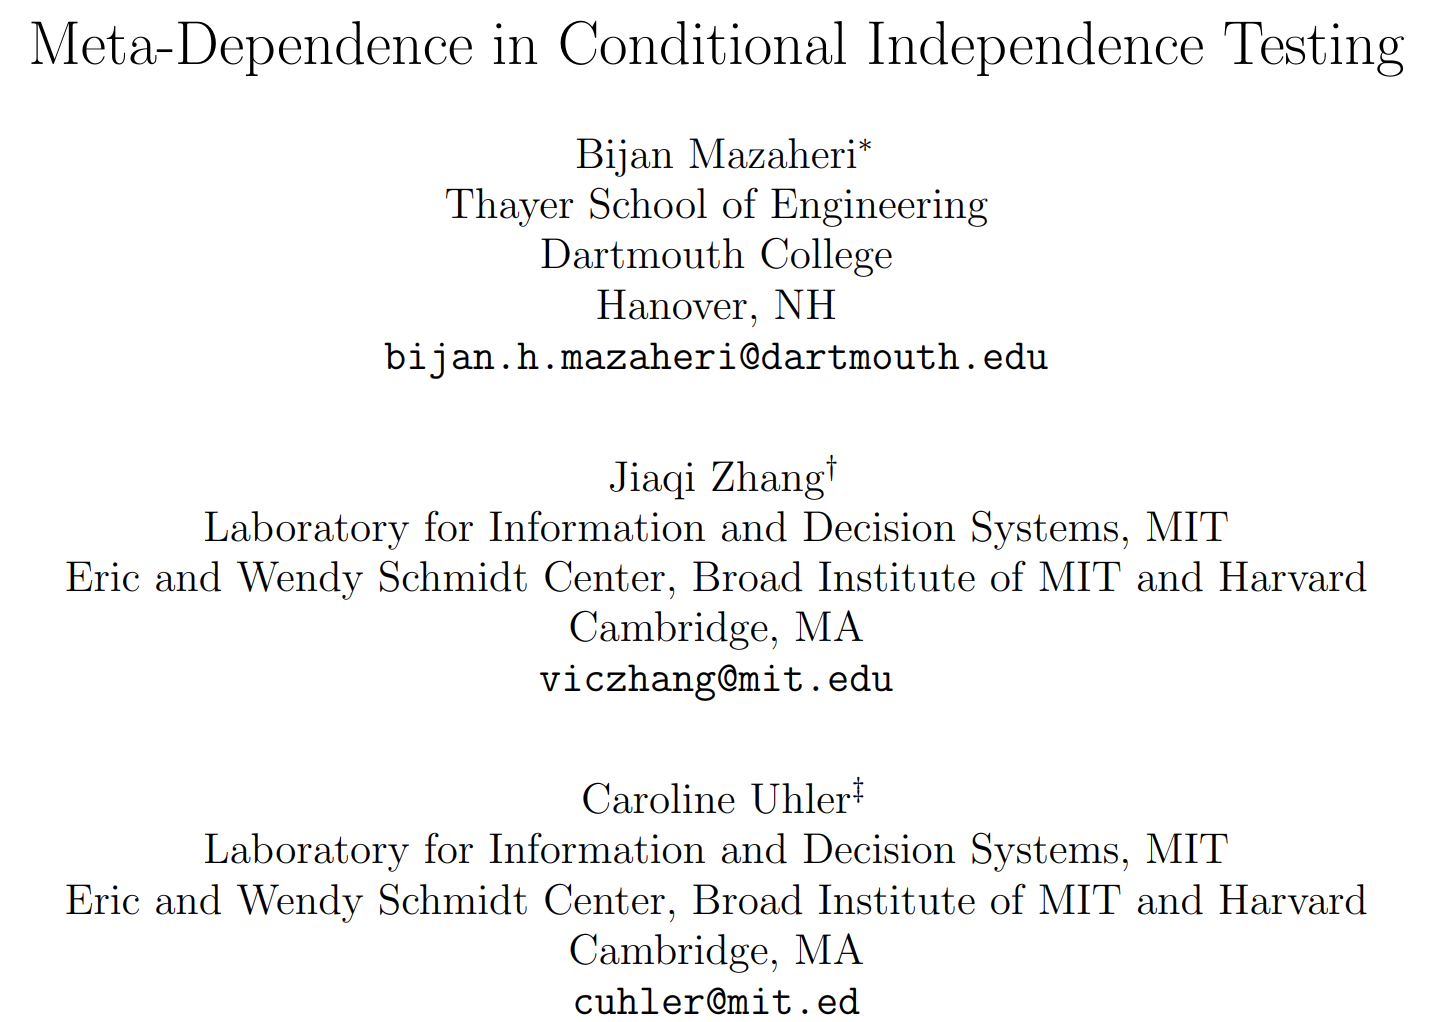
\includegraphics[scale=0.15]{imgs/title.png}
	\end{figure}
\end{frame}

\begin{frame}{Directed Acyclic Graphs (DAGs)}
	\begin{columns}
		\begin{column}{0.55\textwidth}
		\begin{itemize}
			\item Nodes represent random variables.
			\item Edges represent causal relationships.
			\item E.g., \textbf{Education} has a direct effect on \textbf{Income}. 
			\item E.g., \textbf{Age} has indirect effect on \textbf{Income} through \textbf{Education} and \textbf{Hours Per Week}.
			\item Used for causal effect estimation.
		\end{itemize}
		\end{column}

		\begin{column}{0.45 \textwidth}
		\begin{figure}
			\centering
			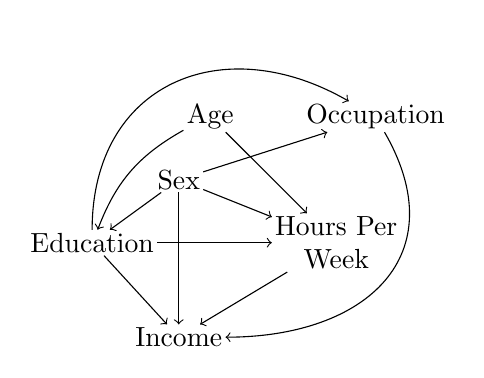
\begin{tikzpicture}[scale=1]
			\tikzstyle{every node}=[align=center, inner sep=1pt]
				\node (sex) at (-0.7, -0.8) {Sex};
				\node (age) at (-0.3, 0) {Age};
				\node (ed) at (-1.8, -1.6) {Education};
				\node (occ) at (1.8, 0) {Occupation};
				\node (hrpw) at (1.3, -1.6) {Hours Per \\ Week};
				\node (income) at (-0.7, -2.8) {Income};
			
				\draw[->]  (age) to[bend right=20] (ed);
				\draw[->]  (sex) to (ed);
				\draw[->]  (age) to (hrpw);
				\draw[->]  (ed) to (hrpw);
				\draw[->]  (sex) to (hrpw);
				\draw[->]  (ed) to (income);
				\draw[->]  (hrpw) to (income);
				\draw[->]  (occ) to[out=300, in=0, looseness=1.4] (income.east);
				\draw[->]  (sex) to (income);
				\draw[->]  (ed) to[out=90, in=150, looseness=1.3] (occ);
				\draw[->]  (sex) to (occ);	
			\end{tikzpicture}
			\caption*{\footnotesize {Example of a DAG}}
		\end{figure}
		\end{column}
	\end{columns}	
\end{frame}

\begin{frame}{Background: Directed Acyclic Graphs}
	\begin{figure}
		\centering
		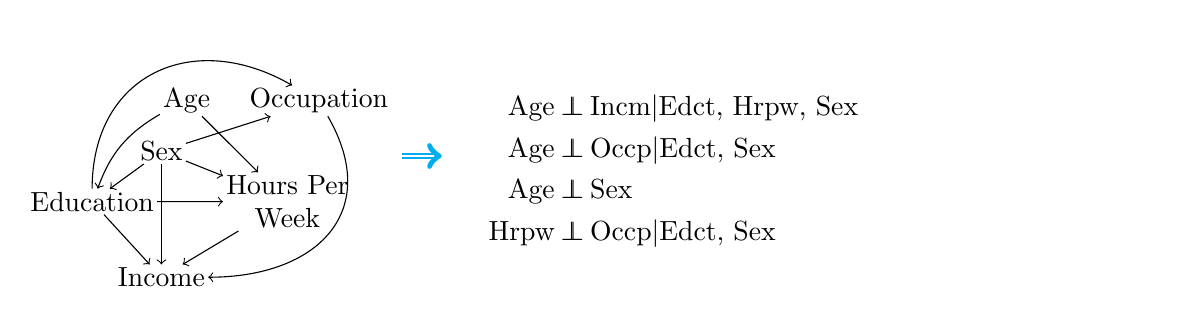
\begin{tikzpicture}
			\begin{scope}[yshift=0.7cm, scale=0.8]
			\tikzstyle{every node}=[align=center, inner sep=1pt]
				\node (sex) at (-0.7, -0.8) {Sex};
				\node (age) at (-0.3, 0) {Age};
				\node (ed) at (-1.8, -1.6) {Education};
				\node (occ) at (1.8, 0) {Occupation};
				\node (hrpw) at (1.3, -1.6) {Hours Per \\ Week};
				\node (income) at (-0.7, -2.8) {Income};
			
				\draw[->]  (age) to[bend right=20] (ed);
				\draw[->]  (sex) to (ed);
				\draw[->]  (age) to (hrpw);
				\draw[->]  (ed) to (hrpw);
				\draw[->]  (sex) to (hrpw);
				\draw[->]  (ed) to (income);
				\draw[->]  (hrpw) to (income);
				\draw[->]  (occ) to[out=300, in=0, looseness=1.4] (income.east);
				\draw[->]  (sex) to (income);
				\draw[->]  (ed) to[out=90, in=150, looseness=1.3] (occ);
				\draw[->]  (sex) to (occ);	
			\end{scope}
			\draw[thick, ->, double, cyan] (2.5,0) -- (3,0);
			\node[rectangle, align=center, inner sep=1pt] at (6, 0) {
				\begin{minipage}{\textwidth}
					\begin{equation*}
						\begin{split}
							\textnormal{Age} &\ci \textnormal{Incm} \rvert \textnormal{Edct, Hrpw, Sex} \\
							\textnormal{Age} &\ci \textnormal{Occp} \rvert \textnormal{Edct, Sex} \\
							\textnormal{Age} &\ci \textnormal{Sex} \\
							\textnormal{Hrpw} &\ci \textnormal{Occp} \rvert \textnormal{Edct, Sex} \\
						\end{split}
					\end{equation*}
				\end{minipage}
				};
		\end{tikzpicture}
	\end{figure}
\end{frame}

\begin{frame}{Causal Discovery: Learning DAGs From Data}
	\vspace{-2em}
	\begin{figure}
		\centering
		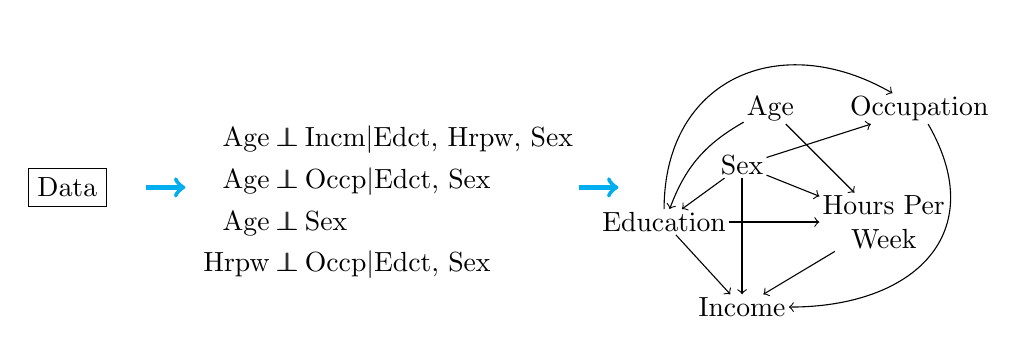
\begin{tikzpicture}
			\node[draw, rectangle] (data) at (0, 0) {Data};
			\draw[ultra thick,->, cyan] (1,0) -- (1.5,0);
			\node[rectangle, align=center, inner sep=1pt] at (3, 0) {
				\begin{minipage}{0.2\textwidth}
					\begin{equation*}
						\begin{split}
							\textnormal{Age} &\ci \textnormal{Incm} \rvert \textnormal{Edct, Hrpw, Sex} \\
							\textnormal{Age} &\ci \textnormal{Occp} \rvert \textnormal{Edct, Sex} \\
							\textnormal{Age} &\ci \textnormal{Sex} \\
							\textnormal{Hrpw} &\ci \textnormal{Occp} \rvert \textnormal{Edct, Sex} \\
						\end{split}
					\end{equation*}
				\end{minipage}
				};
			\begin{scope}[xshift=6.5cm]
				\draw[ultra thick,->,cyan] (0,0) -- (0.5,0);
			\end{scope}	
			\begin{scope}[xshift=9.2cm, yshift=1cm, scale=0.9]
				\tikzstyle{every node}=[align=center, inner sep=1pt]
				\node (sex) at (-0.7, -0.8) {Sex};
				\node (age) at (-0.3, 0) {Age};
				\node (ed) at (-1.8, -1.6) {Education};
				\node (occ) at (1.8, 0) {Occupation};
				\node (hrpw) at (1.3, -1.6) {Hours Per \\ Week};
				\node (income) at (-0.7, -2.8) {Income};
			
				\draw[->]  (age) to[bend right=20] (ed);
				\draw[->]  (sex) to (ed);
				\draw[->]  (age) to (hrpw);
				\draw[->]  (ed) to (hrpw);
				\draw[->]  (sex) to (hrpw);
				\draw[->]  (ed) to (income);
				\draw[->]  (hrpw) to (income);
				\draw[->]  (occ) to[out=300, in=0, looseness=1.4] (income.east);
				\draw[->]  (sex) to (income);
				\draw[->]  (ed) to[out=90, in=150, looseness=1.3] (occ);
				\draw[->]  (sex) to (occ);	
			\end{scope}
		\end{tikzpicture}
	\end{figure}
	\center{Faithfulness: $ X \ci Y | \bm{Z} $ in Data if and only if implied by the DAG.}
\end{frame}

\begin{frame}{Problems with Causal Discovery}
\end{frame}

\begin{frame}{Proposed Solution Summary}
\end{frame}

\begin{frame}{Faithfulness}
\end{frame}

\begin{frame}{$\lambda$-strong Faithfulness}
	\begin{figure}
		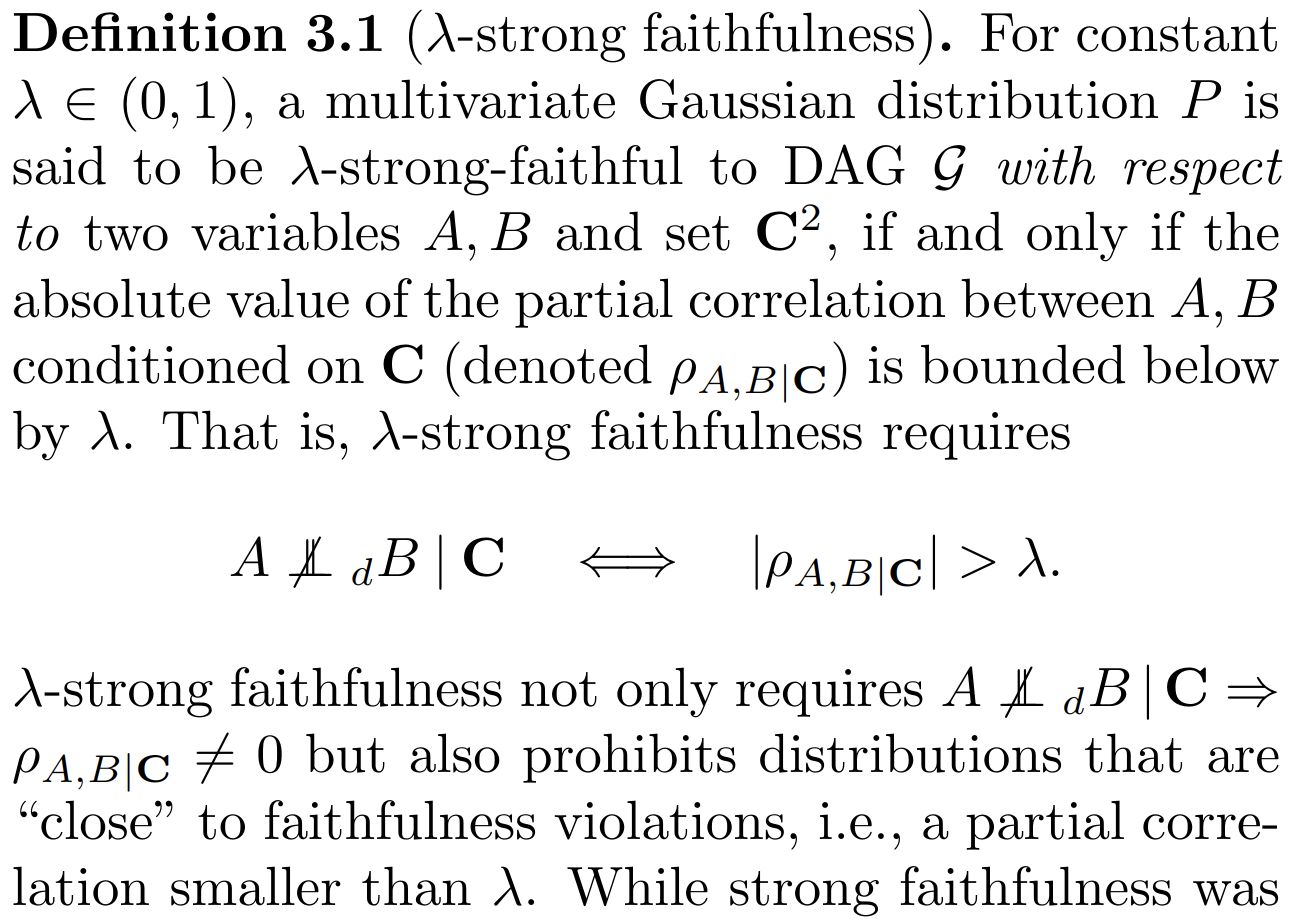
\includegraphics[scale=0.15]{imgs/def31.png}
	\end{figure}
\end{frame}

\begin{frame}{Dependence of Faithfulness}
	\begin{itemize}
		\item Examine the dependence between different faithfulness violations.
		\item Consider a joint distribution $ P $ generated from a DAG $ G $. 
		\item Local parameter perturbations on equation parameters to mimic estimator errors of empirical distributions on finite samples.
		\item Perturbations alter partial correlation between variables resulting in strong faithfulness violations.

	\end{itemize}
\end{frame}

\begin{frame}{Model Setup}
	\begin{itemize}
		\item Linear Additive Gaussian Model: Each variable $V = \sum_{U\in\text{pa}(V)} \theta_{UV}U + N_V$ where $N_V \sim \mathcal N(0,\sigma_V^2)$ and $N_V$’s are mutually independent.
	\end{itemize}
\end{frame}

\begin{frame}{Parameter Perturbations}
	\begin{itemize}
		\item Treat perturbations in the parameter space.
		\item Perturbations move the joint distribution through parameter space towards/away from CI manifolds.
		\item A single perturbation can approach multiple CI manifolds simultaneously.
	\end{itemize}
\end{frame}

\begin{frame}{Parameter Perturbations: Single Violation}
	Consider DAG: $ A \rightarrow B $
	$$ A = N_A, \;\;\; B = \alpha A + N_B $$
	\begin{itemize}
		\item Correlation: $ \rho_{AB} = \alpha $.
		\item The distribution is $ \alpha'$-strong faithful whenever $ \alpha > \alpha' $.
		\item Perturbation: Shift $ \alpha $ to $ \alpha' $ $ \implies $ violation of $ \alpha'$-strong faithfulness.
	\end{itemize}
\end{frame}

\begin{frame}{Parameter Perturbations: Multiple Violations}
	\begin{itemize}
		\item DAG: $ A \rightarrow B \rightarrow C, A \rightarrow C $.
		\item $ A = N_A, \;\;\; B = \alpha_1 A + N_B, \;\;\; C = \alpha_2 A + \beta B + N_C $.
		\item Correlations: $ \rho_{AB} = \alpha_1, \rho_{AC} = \alpha_2 + \alpha_1 \beta , \rho_{BC} = \alpha_1 \alpha_2 + \beta$.
		\item  Assuming DAG: $ A \rightarrow B \rightarrow C $, the distribution is faithful to G if $ A \not \ci B $ and $ A \not \ci C $ implying $ \rho_{AB} \ne 0 $ and $ \rho_{A,C} \ne 0 $.
	\end{itemize}	
\end{frame}

\begin{frame}{Parameter Perturbations: Multiple Violations}
	\begin{itemize}
		\item $ \alpha_1 = 0.5, \alpha_2 = 0.3, \beta = -0.3 $.
		\item Perturb $ \alpha_2 $, $ \rho_{AC} = \alpha_2 - 0.15 = 0.15 $.
	\end{itemize}
\end{frame}


\begin{frame}{Empirical Results}
	\begin{figure}
		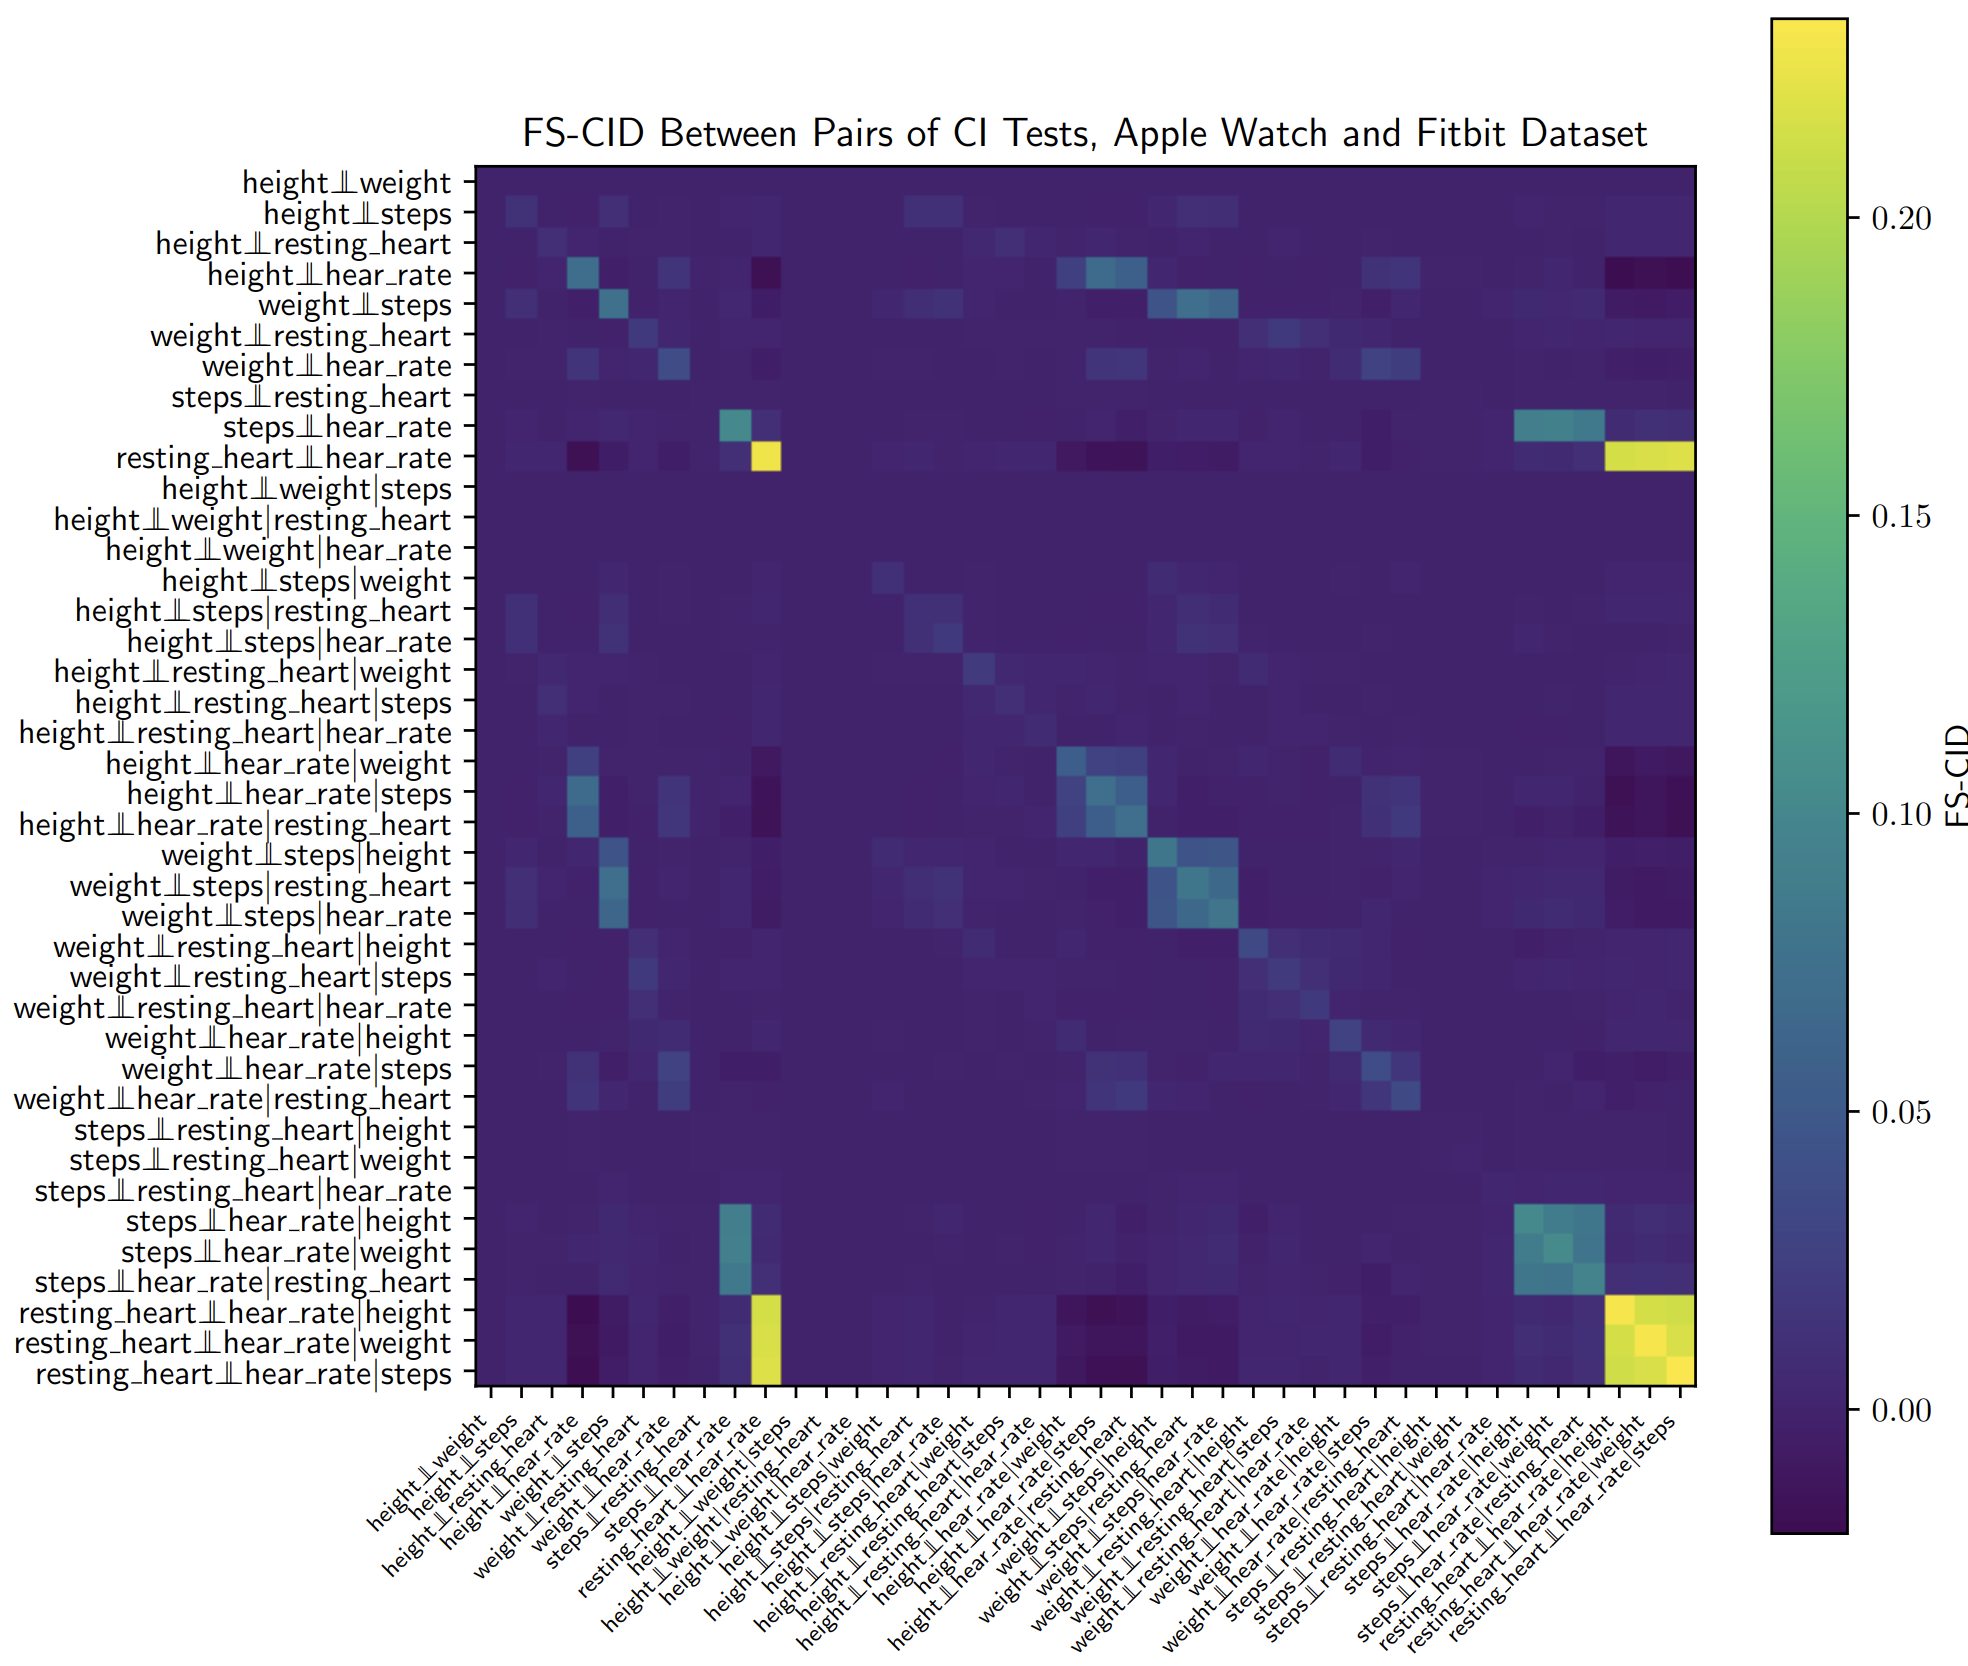
\includegraphics[scale=0.12]{imgs/empirical1.png}
	\end{figure}
\end{frame}

\begin{frame}{Empirical Results}
	\begin{figure}
		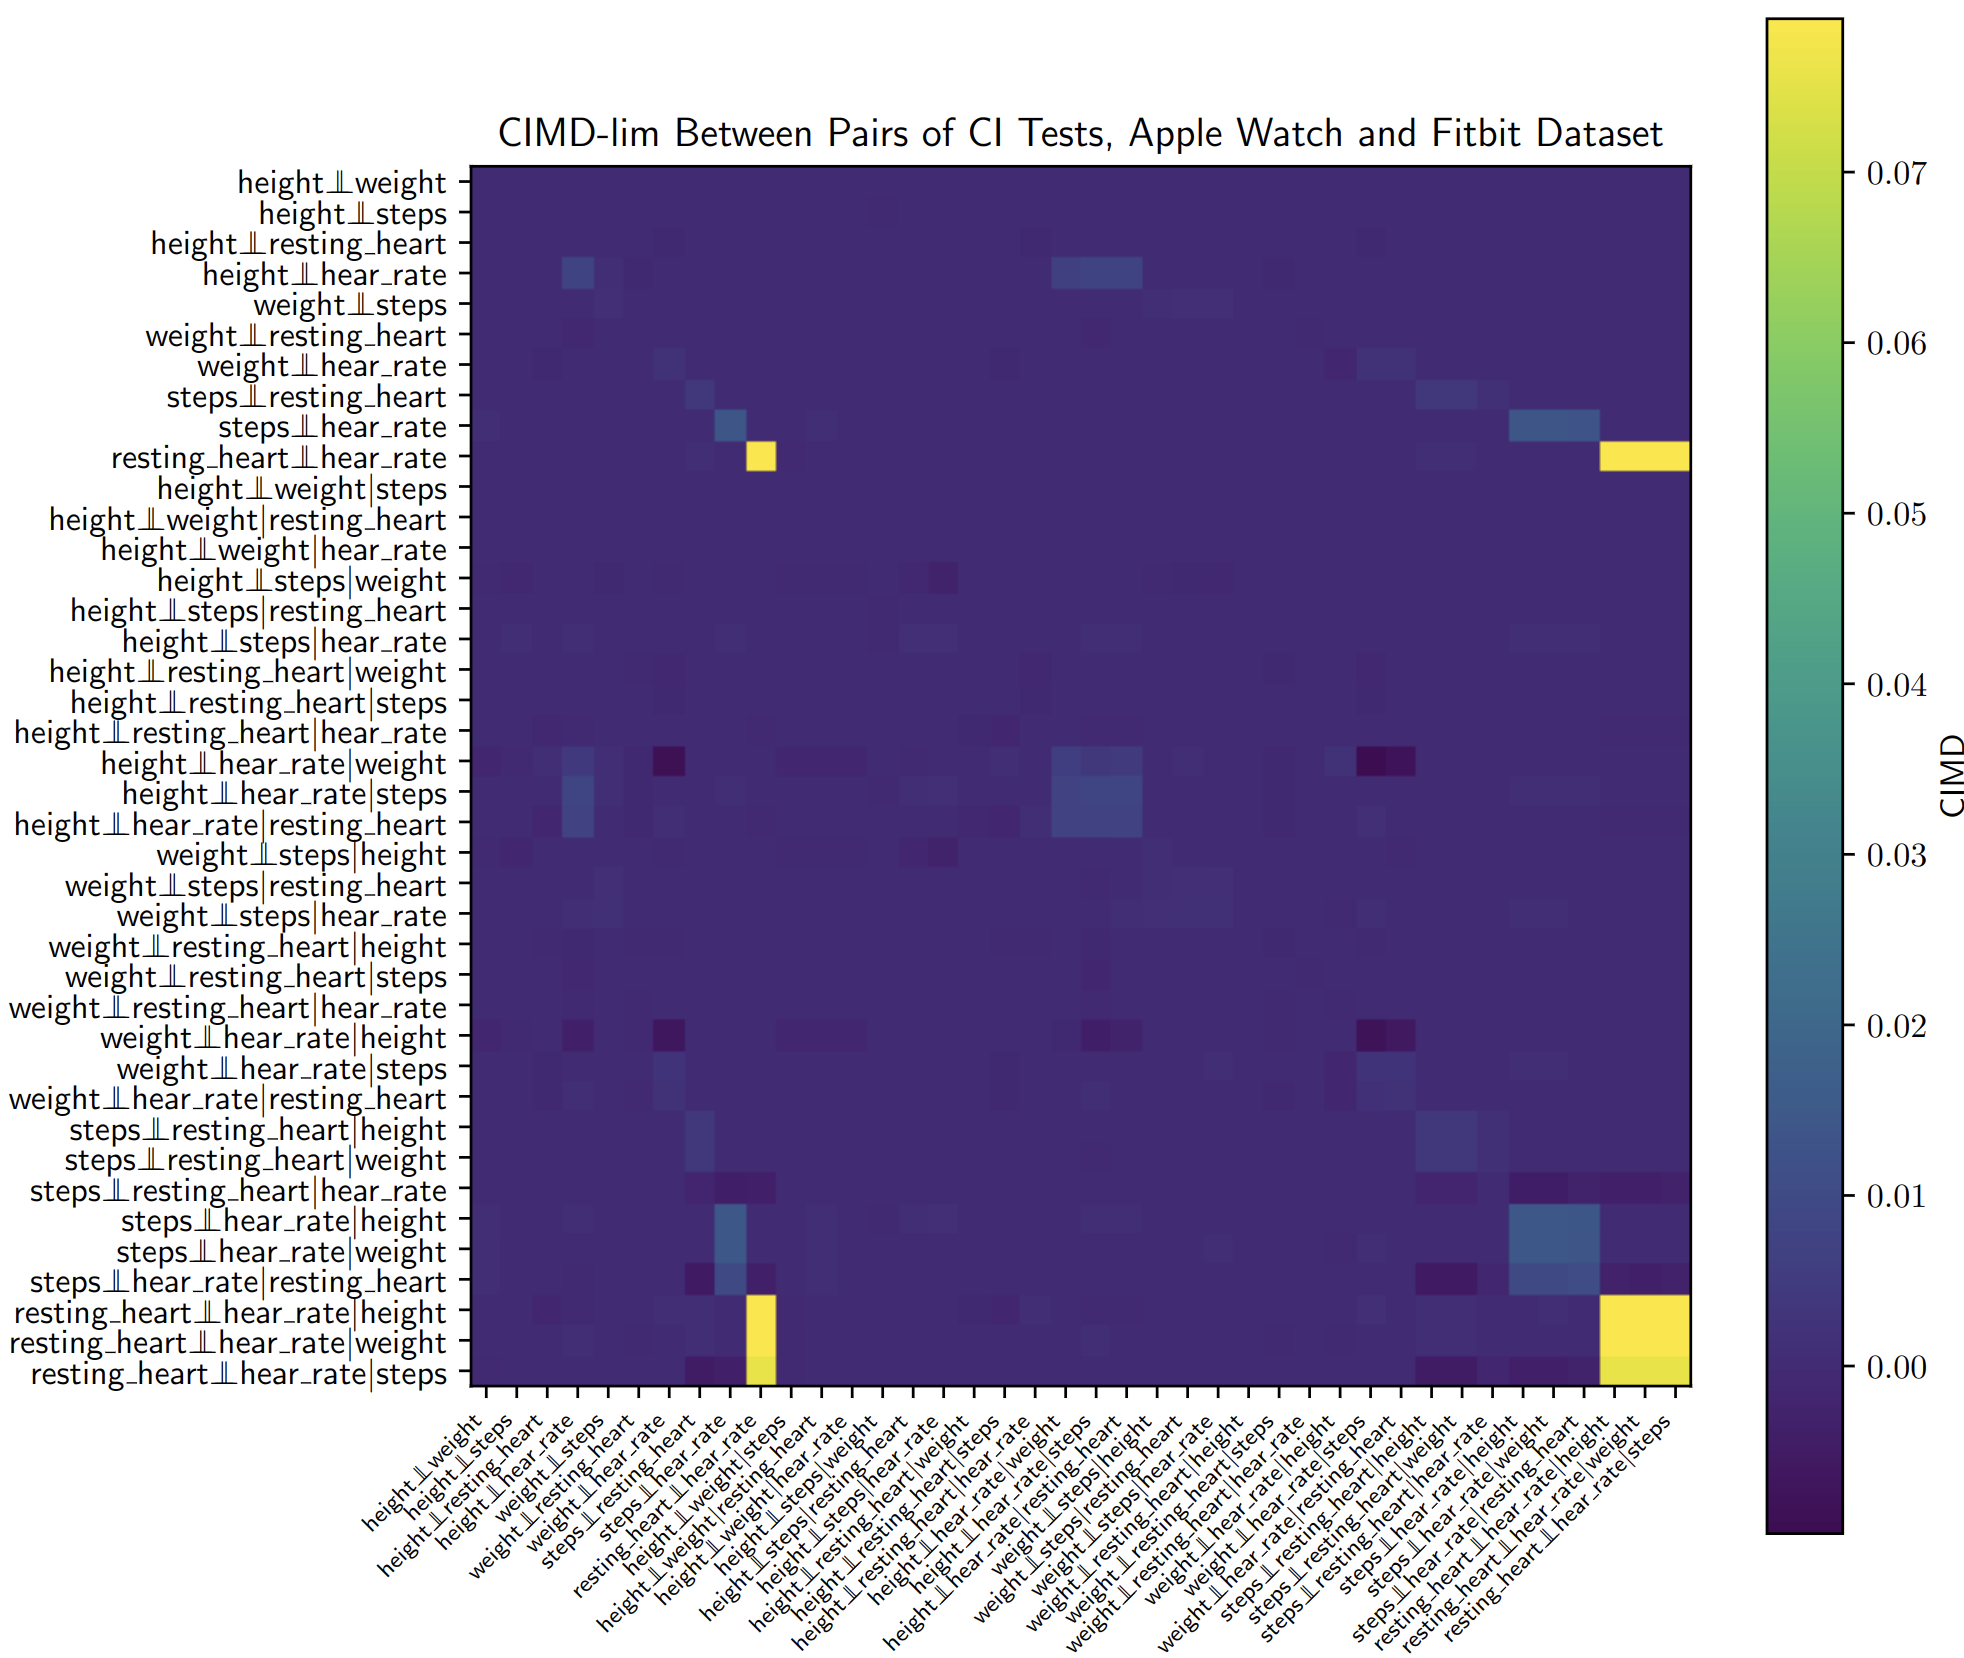
\includegraphics[scale=0.12]{imgs/empirical2.png}
	\end{figure}
\end{frame}

\end{document}
